\section{Аналитическая часть}

В данном разделе рассматриваются понятие оперативной памяти, сжатия данных и ядра Linux. 

\subsection{ЦПУ и оперативная память} 

Оперативная память (\cite{ram}) -- компонент, который позволяет компьютеру кратковременно хранить данные и осуществлять быстрый доступ к ним. Функции оперативной памяти реализуются с помощью специального технического устройства -- оперативного запоминающего устройства (ОЗУ). В этой памяти во время работы компьютера хранится выполняемый машинный код и данные, обрабатываемые центральным процессорным устройством (англ. central processing unit, CPU \cite{cpu}).

В последнее десятилетие центральное процессорное устройство  достигли своей пиковой тактовой частоты -- около 5 Ггц, и этот предел будет преодолён ещё не скоро \cite{cpu_pick}. Из-за того что ЦПУ стали настолько быстрыми, становится нередка ситуация, когда процессор не выполняет инструкции, а ждёт, пока данные переместятся с диска в оперативное запоминающее устройство (или наоборот) \cite{in-kernel-memory-compression}. Так, например, скорость работы системы с мощным ЦПУ, но с маленьким количеством ОЗУ может быть маленькой -- несмотря на быстроту, ЦПУ будет часто будет ожидать подсистему ввода/вывода. \cite{in-kernel-memory-compression}

Проблему объема оперативной памяти компьютера можно решить увеличив количество планок ОЗУ. Но, у данного подхода есть свои минусы:

\begin{itemize}
	\item электроэнергия -- каждая новая установленная планка увеличивает потребление энергии компьютера \cite{increasing-ram-bad};
	\item физические ограничения -- количество слотов для планок на материнской плате ограничено;
	\item стоимость -- планка стоит денег.
\end{itemize}

Альтернативным решением является использование системы подкачки страниц (англ. paging \cite{paging}) -- специальный механизм операционный системы, при котором отдельные фрагменты памяти (мало используемые или полностью не активные) перемещаются из оперативной памяти во вторичной хранилище, например, на жёсткий диск или другой внешний накопитель. Несмотря на то что количество ОЗУ в таком случае увеличивается, доступ к таким участкам памяти замедляется -- системе приходится работать (читать и писать) с внешним запоминающим устройством, а такие устройства работают значительно медленнее ОЗУ \cite{ssd-hdd-speed}.

Ещё одним решением является сжатие данных прямо в оперативной памяти. Данный подход выигрывает у первого рассмотренного решения, так как он реализуется программно и не требует закупки дополнительных планок ОЗУ. Кроме того, этот подход выигрывает и у второго рассмотренного решения, благодаря тому что сжатие не требует работы с внешним накопителем, за счёт чего скорость обработки данных увеличивается. Сжатие данных так же имеет свои минусы, главным из которых является потребность в вычислительных ресурсах. ЦПУ должно выполнять инструкции для сжатия. Но, как и было описано в начале данного раздела, обычно ЦПУ как раз простаивает и не выполняет никакой работы, ожидая ввод/вывод.

\subsection{Сжатие данных}

Сжатие данных (англ. data compression \cite{data-compression}) --  это способ (алгоритмический) преобразования информации в другую форму, обычно более компактную. Сжатие основано на устранение избыточности, которая содержится в исходных данных. Примером является повторение в исходном тексте некоторых фрагментов. Такая избыточность устраняется заменой повторяющейся последовательности ссылкой на уже закодированный фрагмент с указанием его длины. Другой вид избыточности связан с тем, что некоторые значения в сжимаемых данных встречаются чаще других. Сокращение объёма данных достигается за счёт замены часто встречающихся данных короткими кодовыми словами, а редких -- длинными.

Все методы сжатия данных делятся на два класса: без потерь и с потерями. Сжатие данных без потерь позволяет полностью восстановить сжатые данные, в отличии от сжатия с потерями. Первый вариант чаще всего используют для сжатия текстовых данных и компьютерных программ, а сжатие с потерями используют для сокращения аудио- или видеоданных -- для таких данных не требуется полное соответствие исходным данным. Алгоритмы сжатия данных с потерями обладают большей эффективностью, чем алгоритмы без потерь \cite{lossless-compression}.

\subsubsection{Коэффициент сжатия}

Коэффициент сжатия -- характеристика алгоритмов сжатия данных, которая определяется формулой (\ref{fig:memory-compression}): 

\begin{equation}\label{fig:memory-compression}
	k = \frac{V_{original}}{V_{compressed}}
\end{equation}
где $V_{original}$ -- объём исходных данных, а $V_{compressed}$ -- сжатых.

Чем выше коэффициент сжатия, тем алгоритм эффективнее. При этом:

\begin{itemize}
	\item если $k = 1$, то алгоритм сжатия данных не производит. Сжатые данные по размеру равны исходным;
	\item если $k < 1$, то алгоритм сжатия данных создаёт еще больший (по размеру) блок данных, чем исходный.
\end{itemize}

\subsubsection{Требования к алгоритмам сжатия}

К алгоритмам сжатия могут применяться несколько требований:

\begin{itemize}
	\item скорость сжатия;
	\item скорость декомпрессии;
	\item степень сжатия;
	\item эффективность программной реализации.
\end{itemize}

Для каждой конкретной задачи будут важны одни требования и менее важны другие. Так, например, для сжатия больших видеоданных с их последующим хранением, важнее будет степень сжатия данных, а не скорость работы алгоритма.

\subsection{Ядра операционных систем}

Ядро операционной системы -- это программное обеспечение, которое предоставляет базовые функции для всех остальных частей операционной системы, управляет аппаратным обеспечением и распределяет системные ресурсы \cite{kernel-development}. Ядра операционных систем можно разделить на две группы: с монолитным или с микроядром. 

Монолитное ядро является самым простым, оно реализовано в виде одного большого процесса, который выполняется в одном адресном пространстве, все службы ядра находятся и выполняются в одном адресном пространстве. Благодаря этому, взаимодействия в ядре осуществляются очень просто, так, например, ядро может вызывать функции непосредственно, как это делают пользовательские приложения \cite{kernel-development}. Из-за отсутствия издержек, таких как синхронизация процессов и передача данных между ними, монолитные ядра операционных систем являются более производительным, чем микроядра. На рисунке \ref{fig:monolithic kernel} представлена концептуальная схема операционной системы с монолитном ядром.

\begin{figure}[h]
	\centering
	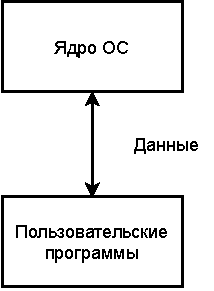
\includegraphics[scale=2]{img/monolithic_kernel.pdf}
	\caption{Схема ОС с монолитным ядром}
	\label{fig:monolithic kernel}
\end{figure}
 
Реализация микроядра подразумевает отказ от одного большого процесса. Все функции ядра разделяются на несколько процессов, которые обычно называют серверами \cite{kernel-development}. При этом, в привилегированном режиме могут работать лишь те сервера (процессы), которым этот режим необходим, а остальные сервера работают в непривилегированном (пользовательском) режиме. К первым типам процессов можно отнести, например, механизмы управления памятью компьютера, а ко вторым драйвера устройств. При таком подходе все сервера изолированы и работают в независящем друг от друга адресном пространстве, то есть прямой вызов функций (как в монолитном ядре) невозможен. Все взаимодействия между серверами происходит с помощью механизма межпроцессного взаимодействия (англ. Interprocess Communcation, IPC \cite{IPC}), а обеспечивает передачу данных само ядро (больше никаких действий в системе оно не выполняет). Такой подход позволяет предотвратить возможность выхода из строя одного сервера при выходе из строя другого и позволяет по по мере необходимости одному серверу выгрузить из памяти другой. Но, как уже было отмечено выше, такая модель имеет более низкую производительность из-за накладных расходов на IPC. На рисунке \ref{fig:micro_kernel} представлена концептуальная схема операционной системы с монолитном ядром. 

\begin{figure}[h]
	\centering
	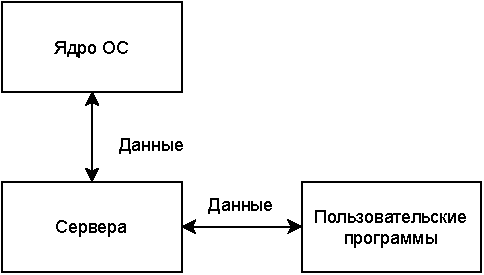
\includegraphics[width=\textwidth]{img/micro_kernel.pdf}
	\caption{Схема ОС с микроядром}
	\label{fig:micro_kernel}
\end{figure}

\subsection{Ядро Linux}

Ядро Linux \cite{linux} -- ядро операционной системы с открытым исходным кодом, распространяющееся как свободное программное обеспечение. Именно из-за этого в данной работе будет рассмотрено данное ядро. Ядро Linux является монолитным. Но, несмотря на это, при разработке ядра была из микроядерной модели были позаимствованы некоторые решения: модульный принцип построения, приоритетное планирование самого себя, поддержка многопоточного режима и динамической загрузки в ядро внешних бинарных файлов (модулей ядра) \cite{kernel-development}. Linux не использует никаких функций микроядерной модели (IPC), которые приводят к снижению производительности системы.

Ниже представлены отличительные черты ядра Linux:

\begin{itemize}
	\item потоки ничем не отличаются от обычных процессов. С точки зрения ядра все процессы одинаковы и лишь некоторые из них делят ресурсы между собой;
	\item динамическая загрузка модулей ядра;
	\item приоритетное планирование. Ядро способно прервать выполнение текущего процесса, даже если оно выполняется в режиме ядра;
	\item объектно-ориентированная модель устройств. Ядро поддерживает классы устройств и события;
	\item ядро Linux является результатом свободной и открытой модели разработки \cite{kernel-development}.
\end{itemize}

\subsubsection{Структура ядра}

Ядро Linux состоит из нескольких основных компонентов:

\begin{itemize}
	\item планировщик процессов -- определяет, какой из процессов должен выполняться, в какой момент и как долго;
	\item менеджер памяти -- обеспечивает работу виртуальной памяти и непосредственно доступ к ней;
	\item виртуальная файловая система -- специальный единый файловый интерфейс, скрывающий интерфейс физических устройств;
	\item сетевые интерфейсы -- обеспечивают работу с сетевым оборудованием;
	\item межпроцессная подсистема -- механизмы межпроцессного взаимодействия.
\end{itemize}

\subsubsection{Виртуальная память}

Виртуальная память -- специальный механизм организации памяти, при котором процессы работают физическими адресами напрямую, а с виртуальными. С помощью такого подхода в ядре Linux реализуется защита адресного пространства процессов, так, например, процесс не может получить доступ к памяти другого процесса и внести туда изменения.

Работа с память в ядре Linux организована с помощью примитива страниц. Страница памяти -- набор некоторого количества байт. Хотя наименьшими адресуемыми единицами памяти являются байт и машинное слово, такой подход не является удобным \cite{kernel-development}. 

В ядре каждая физическая страница памяти представляется в виде структуры \texttt{struct page}. Рассматриваемая структура с наиболее важными полями представлена в листинге \ref{code:struct_page}.

\begin{code}
	\captionof{listing}{Структура \texttt{struct page}}
	\label{code:struct_page}
	\inputminted
	[
	frame=single,
	framerule=0.5pt,
	framesep=20pt,
	fontsize=\small,
	tabsize=4,
	linenos,
	numbersep=5pt,
	xleftmargin=10pt,
	]
	{text}
	{code/struct_page.c}
\end{code}

Рассмотрим некоторые поля данной структуры подробнее:

\begin{itemize}
	\item \texttt{flags} -- флаги, которые хранят информацию о состоянии страницы в текущий момент, например, находится ли данная страница в кэше или нет. Каждый флаг представляет из себя один бит;
	\item \texttt{\_refcount} -- счётчик ссылок на страницу. Если значение этого счётчика равно -1, это означает что страница нигде не используется;
	\item \texttt{virtual} -- виртуальный адрес страницы, соответствует адресу страницы в виртуальной памяти ядра.
\end{itemize}

Рассматриваемая структура данных в ядре используется для учёта всей физической памяти, и определения какая область (страницы) памяти свободна, а какая нет. 

В ядре Linux предусмотрен специальный низкоуровневый механизм для выделения памяти и несколько интерфейсов доступа к ней. Прототип функции основной функции выделения памяти представлен в листинге \ref{code:alloc_pages}.

\begin{code}
	\captionof{listing}{Прототип функции \texttt{alloc\_pages}}
	\label{code:alloc_pages}
	\inputminted
	[
	frame=single,
	framerule=0.5pt,
	framesep=20pt,
	fontsize=\small,
	tabsize=4,
	linenos,
	numbersep=5pt,
	xleftmargin=10pt,
	]
	{text}
	{code/alloc_pages.c}
\end{code}

С помощью функции \texttt{alloc\_pages} можно выделить $2^{order}$ смежных страниц физической памяти. Возвращает указатель на структуру \texttt{struct page}, которая соответствует первой выделенной странице памяти. Для выделения одной страницы памяти используется функция \texttt{alloc\_page} (листинг \ref{code:alloc_page}).

\begin{code}
	\captionof{listing}{Прототип функции \texttt{alloc\_page}}
	\label{code:alloc_page}
	\inputminted
	[
	frame=single,
	framerule=0.5pt,
	framesep=20pt,
	fontsize=\small,
	tabsize=4,
	linenos,
	numbersep=5pt,
	xleftmargin=10pt,
	]
	{text}
	{code/alloc_page.c}
\end{code}

\subsubsection{Сжатие памяти в ядре Linux}

Для сжатия данных в оперативной памяти, ядро берёт последовательность байт в памяти, сжимает их, записывает сжатую версию обратно в ОЗУ и хранит их до тех пор, пока эти данные не потребуются системе. Пока данные находятся в сжатом состоянии, система не может прочитать или записать какие-либо отдельные байты из этой сжатой последовательности. Когда данные потребуется системе вновь, система восстанавливает сжатую последовательность.

Современные алгоритмы могут сжимать любое количество последовательных байт. Несмотря на это, в ядре удобно использовать фиксированную единицу сжатия памяти. Единицей хранения в ядре была выбрана страница памяти (англ. memory page \cite{memory-page}) -- фиксированная константа \texttt{PAGE\_SIZE}, которая на большинстве современных архитектур, поддерживаемых Linux, составляет 4 Кб \cite{4kb-page-size}.

Для достижения высокой степени сжатия требуется выполнение большого количества команд ЦПУ, тогда как менее эффективное сжатие может выполняться быстрее. В ядре необходимо добиться баланса между временем и степенью сжатия. Кроме того, важно чтобы выбор алгоритма оставался гибким. Например для выполнения одной задачи подойдёт один алгоритм сжатия, а для второй другой.

Из-за того что размер страницы достаточно большой (4 Кб), сжатие и восстановление данных -- достаточно дорогостоящие операции, поэтому необходимо ограничить количество этих операций. Нужно тщательно выбирать, какие страницы стоит сжимать, а какие нет. Алгоритм, реализованный в ядре Linux, определяющий какие страницы нужно сжимать, выбирает те страницы, которые вероятно будут использоваться снова, но вряд ли будут использоваться в ближайшем будущем \cite{in-kernel-memory-compression}. Такая реализация позволяет не тратить всё время ЦПУ на многократное сжатие и распаковку страниц. Кроме того, необходимо чтобы ядро могло идентифицировать сжатую страницу -- иначе её невозможно найти и распаковать.

Размер страницы, к которой был применён алгоритм сжатия зависит от данных на исходной странице и его трудно предсказать. Степень сжатия страницы описывается следующей формулой (\ref{fig:page-compressing}):

\begin{equation}\label{fig:page-compressing}
	k = \frac{PAGE\_SIZE}{zsize}
\end{equation}
где \texttt{PAGE\_SIZE} размер страницы памяти в системе, а \texttt{zsize} -- размер сжатой страницы. 

Обычно размер сжатой страницы меньше чем \texttt{PAGE\_SIZE}, поэтому, обычно, коэффициент сжатия меньше единицы. Но, в некоторых случаях, коэффициент сжатия может быть больше единицы, и для решения этой проблемы необходимо, чтобы алгоритм реализованный в ядре мог найти выход из такой ситуации. В среднем страница памяти в ядре сжимается в два раза \cite{in-kernel-memory-compression}, то есть коэффициент сжатия $ k =\frac{1}{2}$.

\subsubsection{Модуль zRam}

zRam \cite{zRam} -- модуль ядра Linux, который использует сжатое блочное устройство в оперативной памяти, пока не появится необходимость использовать файл подкачки (swap) на жестком диске. Данный модуль поддерживает несколько алгоритмов сжатия (на выбор пользователя), например DEFLATE, LZ0, LZ4, ZSTD. Модуль zRam описывается одним экземпляром структуры \texttt{struct zram} (листинг \ref{code:zram})

\begin{code}
	\captionof{listing}{Структура \texttt{struct zram}}
	\label{code:zram}
	\inputminted
	[
	frame=single,
	framerule=0.5pt,
	framesep=20pt,
	fontsize=\small,
	tabsize=4,
	linenos,
	numbersep=5pt,
	xleftmargin=10pt,
	]
	{text}
	{code/zram.c}
\end{code}

Рассматриваемая структура хранит в себе таблицу страниц, семафор, с помощью которого достигается синхронизация при параллельной обработке \cite{in-kernel-memory-compression}, название алгоритма, которые будет производить сжатие, размер диска, статистику и другие поля.

Для хранения информации о сжатых страницах (их размер и данные) используется специальная таблица. Это необходимо, для того чтобы найти эту страницу для её дальнейшего преобразования к исходному (не сжатому) виду. Для этого используется структура \texttt{struct zram\_table\_entry}, которая представлена в листинге \ref{code:zram_table_entry}

\begin{code}
	\captionof{listing}{Структура \texttt{struct zram\_table\_entry}}
	\label{code:zram_table_entry}
	\inputminted
	[
	frame=single,
	framerule=0.5pt,
	framesep=20pt,
	fontsize=\small,
	tabsize=4,
	linenos,
	numbersep=5pt,
	xleftmargin=10pt,
	]
	{text}
	{code/zram_table_entry.c}
\end{code}

Для идентификации страниц и управления данными данный модуль использует прямой поиск по таблице страниц (массив из структур \\\texttt{struct zram\_table\_entry}), которая хранится в структуре \texttt{struct zram}.

Параллельная обработка страниц ограничивается семафором \\\texttt{struct rw\_semaphore}.


\pagebreak
